\documentclass[10pt]{beamer}
\usetheme{Combo}
\usepackage[utf8]{inputenc}
\usepackage[english]{babel}
\usepackage{graphicx}
\usepackage{tikz}
\usepackage{amsmath}
\usetikzlibrary{shapes,arrows,positioning}
\author{Giovanni Bacci}
\title{Mining Microbiomes}
\subtitle{Computational Biology approaches to uncover the complexity of bacterial communities}
\institute{University of Florence\\
CRA-RPS}
\date{February 10, 2015}
%\setbeamercovered{transparent} 
%\setbeamertemplate{navigation symbols}{} 
%\logo{} 
%\date{} 
%\subject{} 
\begin{document}

\begin{frame}[plain]
\titlepage
\end{frame}

%%%%%%%%%%%%%%%%%%%%%%%%%%%%%%%%%%%%%%%%%%%%%%%%%%%%%%%%%%%%%%%%%%%%%%%%%%%%%%%%%%%%%%%%%%%%%%%%%%%%%%%%%%%%%%%%%%%%%%%%%%%%%%%%%%%
%%% START - BACKGROUND
%%%%%%%%%%%%%%%%%%%%%%%%%%%%%%%%%%%%%%%%%%%%%%%%%%%%%%%%%%%%%%%%%%%%%%%%%%%%%%%%%%%%%%%%%%%%%%%%%%%%%%%%%%%%%%%%%%%%%%%%%%%%%%%%%%%
\section{Background}
\subsection{}

%%%%%%%%%%%%%%%%%%%%%%%%%%%%%%%%%%%%%%%%%%%%%%%%%%%%%%%%%%%%%%%%%%%%%%%%%%%%%%%%%%%%%%%%%%%%%%%%%%%%%%%%%%%%%%%%%%%%%%%%%%%%%%%%%%%
%%% START - Slide 1 
%%%%%%%%%%%%%%%%%%%%%%%%%%%%%%%%%%%%%%%%%%%%%%%%%%%%%%%%%%%%%%%%%%%%%%%%%%%%%%%%%%%%%%%%%%%%%%%%%%%%%%%%%%%%%%%%%%%%%%%%%%%%%%%%%%%
\begin{frame}
\vspace{4mm}
\begin{center}
	{\Large\textbf{A bacterial World...}}
\end{center}
\vspace{-2mm}
		\begin{center}
			\begin{overlayarea}{1\textwidth}{0.2\textheight}
			\only<1>{
			\begin{block}{}
				\begin{center}
					Bacteria are often cited as examples of one of the Earth’s most primitive living forms		
				\end{center}
			\end{block}
			}
			\only<2>{
			\begin{block}{}
				\begin{center}
					They have been always considered from an anthropocentric perspective
				\end{center}
			\end{block}
			}
			\only<3>{
			\begin{block}{}
				\begin{center}
					They are still associated almost exclusively to infection diseases
				\end{center}
			\end{block}
			}
			\only<4>{
			\begin{block}{}
				\begin{center}
					They are often studied to develop new antibiotic treatments
				\end{center}
			\end{block}
			}
			\only<5>{
			\begin{block}{}
				\begin{center}
					But reality is rather different
				\end{center}
			\end{block}
			}
			\only<6>{
			\begin{block}{}
				\begin{center}
					Only a very small fraction of bacteria is able to cause infections
				\end{center}
			\end{block}
			}
			\only<7>{
			\begin{block}{}
				\begin{center}
					A highly diversified and beneficial bacterial world exists
				\end{center}
			\end{block}
			}
			\end{overlayarea}
		\end{center}
		\begin{center}
			\begin{overlayarea}{1\textwidth}{0.6\textheight}
			\only<1>{\begin{center}\includegraphics[width=0.8\textwidth]{./images/bacwcartoon/bacterial_world1-01}\end{center}}
			\only<2>{\begin{center}\includegraphics[width=0.8\textwidth]{./images/bacwcartoon/bacterial_world2-01}\end{center}}
			\only<3>{\begin{center}\includegraphics[width=0.8\textwidth]{./images/bacwcartoon/bacterial_world3-01}\end{center}}
			\only<4>{\begin{center}\includegraphics[width=0.8\textwidth]{./images/bacwcartoon/bacterial_world4-01}\end{center}}
			\only<5>{\begin{center}\includegraphics[width=0.8\textwidth]{./images/bacwcartoon/bacterial_world5-01}\end{center}}
			\only<6>{\begin{center}\includegraphics[width=0.8\textwidth]{./images/bacwcartoon/bacterial_world6-01}\end{center}}
			\only<7>{\begin{center}\includegraphics[width=0.8\textwidth]{./images/bacwcartoon/bacterial_world7-01}\end{center}}	
			\end{overlayarea}		
		\end{center}
\end{frame}
%%%%%%%%%%%%%%%%%%%%%%%%%%%%%%%%%%%%%%%%%%%%%%%%%%%%%%%%%%%%%%%%%%%%%%%%%%%%%%%%%%%%%%%%%%%%%%%%%%%%%%%%%%%%%%%%%%%%%%%%%%%%%%%%%%%
%%% END - Slide 1 
%%%%%%%%%%%%%%%%%%%%%%%%%%%%%%%%%%%%%%%%%%%%%%%%%%%%%%%%%%%%%%%%%%%%%%%%%%%%%%%%%%%%%%%%%%%%%%%%%%%%%%%%%%%%%%%%%%%%%%%%%%%%%%%%%%%

%%%%%%%%%%%%%%%%%%%%%%%%%%%%%%%%%%%%%%%%%%%%%%%%%%%%%%%%%%%%%%%%%%%%%%%%%%%%%%%%%%%%%%%%%%%%%%%%%%%%%%%%%%%%%%%%%%%%%%%%%%%%%%%%%%%
%%% START - Slide 2
%%%%%%%%%%%%%%%%%%%%%%%%%%%%%%%%%%%%%%%%%%%%%%%%%%%%%%%%%%%%%%%%%%%%%%%%%%%%%%%%%%%%%%%%%%%%%%%%%%%%%%%%%%%%%%%%%%%%%%%%%%%%%%%%%%%
\begin{frame}
	\begin{overlayarea}{1\textwidth}{0.9\textheight}
	\only<1>{\begin{center}\includegraphics[width=0.7\textwidth]{./images/diversity/div-1.eps}\end{center}}
	\only<2>{\begin{center}\includegraphics[width=0.7\textwidth]{./images/diversity/div-2.eps}\end{center}}
	\only<3->{\begin{center}\includegraphics[width=0.7\textwidth]{./images/diversity/div-3.eps}\end{center}}
	\vspace{-2mm}
	\only<4->{
	\begin{block}{}	
	\begin{center}
		\textit{Metagenomics (also referred to as environmental and community genomics) is the genomic analysis of microorganisms by direct extraction and cloning of DNA from an assemblage of microorganisms.}\\
		\hfill\cite{handelsman2004metagenomics}
	\end{center}		
	\end{block}
	}
	\end{overlayarea}
\end{frame}
%%%%%%%%%%%%%%%%%%%%%%%%%%%%%%%%%%%%%%%%%%%%%%%%%%%%%%%%%%%%%%%%%%%%%%%%%%%%%%%%%%%%%%%%%%%%%%%%%%%%%%%%%%%%%%%%%%%%%%%%%%%%%%%%%%%
%%% END - Slide 2
%%%%%%%%%%%%%%%%%%%%%%%%%%%%%%%%%%%%%%%%%%%%%%%%%%%%%%%%%%%%%%%%%%%%%%%%%%%%%%%%%%%%%%%%%%%%%%%%%%%%%%%%%%%%%%%%%%%%%%%%%%%%%%%%%%%

%%%%%%%%%%%%%%%%%%%%%%%%%%%%%%%%%%%%%%%%%%%%%%%%%%%%%%%%%%%%%%%%%%%%%%%%%%%%%%%%%%%%%%%%%%%%%%%%%%%%%%%%%%%%%%%%%%%%%%%%%%%%%%%%%%%
%%% START - Slide 3
%%%%%%%%%%%%%%%%%%%%%%%%%%%%%%%%%%%%%%%%%%%%%%%%%%%%%%%%%%%%%%%%%%%%%%%%%%%%%%%%%%%%%%%%%%%%%%%%%%%%%%%%%%%%%%%%%%%%%%%%%%%%%%%%%%%
\begin{frame}
	\begin{columns}
		
		\begin{column}{0.5\textwidth}
			\vspace{-2mm}
			\begin{center}
				\Large\textbf{Great plate count anomaly}	
			\end{center}
			\begin{center}			
			\includegraphics[width=\textwidth]{./images/Great-plate-count-anomaly}
			\end{center}
		\end{column}
		
		\begin{column}{0.5\textwidth}
			\begin{overlayarea}{0.9\textwidth}{0.9\textheight}
			\vspace{1mm}				
			\small{%
				\only<1->{%
				\begin{center}
					Counts of cells obtained via cultivation are orders of magnitude lower than those directly observed via microscope \cite{staley1985measurement}
				\end{center}}%
				\only<2->{%
				\begin{alertblock}{}				
				\begin{center}
					Using standard laboratory techniques, microbiologists are able to cultivate only 1\% of existent bacteria \cite{hugenholtz2002exploring}				
				\end{center}					
				\end{alertblock}}%				
			}%
			\begin{center}			
				\only<3->{\includegraphics[width=0.9\textwidth]{./images/metagenomics}}
			\end{center}
			\end{overlayarea}
		\end{column}
		
	\end{columns}
\end{frame}
%%%%%%%%%%%%%%%%%%%%%%%%%%%%%%%%%%%%%%%%%%%%%%%%%%%%%%%%%%%%%%%%%%%%%%%%%%%%%%%%%%%%%%%%%%%%%%%%%%%%%%%%%%%%%%%%%%%%%%%%%%%%%%%%%%%
%%% END - Slide 3
%%%%%%%%%%%%%%%%%%%%%%%%%%%%%%%%%%%%%%%%%%%%%%%%%%%%%%%%%%%%%%%%%%%%%%%%%%%%%%%%%%%%%%%%%%%%%%%%%%%%%%%%%%%%%%%%%%%%%%%%%%%%%%%%%%%

%%%%%%%%%%%%%%%%%%%%%%%%%%%%%%%%%%%%%%%%%%%%%%%%%%%%%%%%%%%%%%%%%%%%%%%%%%%%%%%%%%%%%%%%%%%%%%%%%%%%%%%%%%%%%%%%%%%%%%%%%%%%%%%%%%%
%%% START- Slide 4
%%%%%%%%%%%%%%%%%%%%%%%%%%%%%%%%%%%%%%%%%%%%%%%%%%%%%%%%%%%%%%%%%%%%%%%%%%%%%%%%%%%%%%%%%%%%%%%%%%%%%%%%%%%%%%%%%%%%%%%%%%%%%%%%%%%
\begin{frame}
	\begin{overlayarea}{\textwidth}{0.95\textheight}
		\only<1>{%
			\begin{center}
				\includegraphics[width=0.93\textwidth]{./images/uber_pipeline_01}
			\end{center}}%
		\only<2>{%
			\begin{center}
				\includegraphics[width=0.93\textwidth]{./images/uber_pipeline_02}
				\vspace{-5cm}
				\begin{columns}
					\begin{column}{0.3\textwidth}
					% Nothing here
					\end{column}
					\begin{column}{0.3\textwidth}
						\begin{center}						
						\begin{alertblock}{}
						\begin{center}
							All approaches are based on high throughput sequencing technologies					
						\end{center}					
						\end{alertblock}
						\end{center}
					\end{column}	
					\begin{column}{0.4\textwidth}
					% Nothing here
					\end{column}
				\end{columns}			
			\end{center}}%	
	\end{overlayarea}		
\end{frame}
%%%%%%%%%%%%%%%%%%%%%%%%%%%%%%%%%%%%%%%%%%%%%%%%%%%%%%%%%%%%%%%%%%%%%%%%%%%%%%%%%%%%%%%%%%%%%%%%%%%%%%%%%%%%%%%%%%%%%%%%%%%%%%%%%%%
%%% END - Slide 4
%%%%%%%%%%%%%%%%%%%%%%%%%%%%%%%%%%%%%%%%%%%%%%%%%%%%%%%%%%%%%%%%%%%%%%%%%%%%%%%%%%%%%%%%%%%%%%%%%%%%%%%%%%%%%%%%%%%%%%%%%%%%%%%%%%%

%%%%%%%%%%%%%%%%%%%%%%%%%%%%%%%%%%%%%%%%%%%%%%%%%%%%%%%%%%%%%%%%%%%%%%%%%%%%%%%%%%%%%%%%%%%%%%%%%%%%%%%%%%%%%%%%%%%%%%%%%%%%%%%%%%%
%%% START - Slide 5
%%%%%%%%%%%%%%%%%%%%%%%%%%%%%%%%%%%%%%%%%%%%%%%%%%%%%%%%%%%%%%%%%%%%%%%%%%%%%%%%%%%%%%%%%%%%%%%%%%%%%%%%%%%%%%%%%%%%%%%%%%%%%%%%%%%
\begin{frame}
	\vspace{-6mm}
	\begin{overlayarea}{\textwidth}{\textheight}
	\begin{block}{DNA sequencing timeline}
	\begin{center}
	%\large\textbf{{DNA sequencing timeline}}
	\scriptsize{
	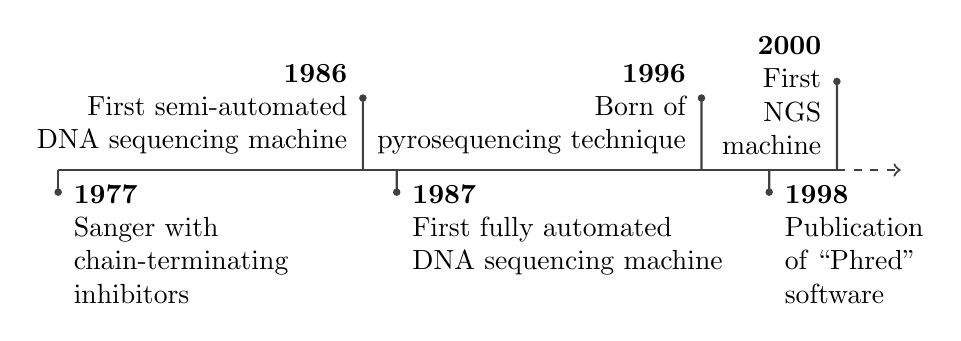
\begin{tikzpicture}
	
		% Vertical lines (all the same)
		%\foreach \x in {0, 3.87, 4.30, 8.17, 9.03, 9.89}
		%\draw [darkgray, thick] (\x cm,3pt) -- (\x cm,-3pt);
		
		% Vertical lines all different
		% 1977 - 0x down
		\draw [darkgray, thick] (0,0) -- (0cm,-8pt);
		\draw [darkgray, fill] (0cm, -8pt) circle [radius=0.04];
		
		% 1986 - 3.87x up
		\draw [darkgray, thick] (3.87,0) -- (3.87cm, 26pt);
		\draw [darkgray, fill] (3.87cm, 26pt) circle [radius=0.04];
		
		% 1987 - 4.30x down
		\draw [darkgray, thick] (4.30,0) -- (4.30cm,-8pt);
		\draw [darkgray, fill] (4.30cm, -8pt) circle [radius=0.04];
		
		% 1996 - 8.17x up
		\draw [darkgray, thick] (8.17,0) -- (8.17cm, 26pt);
		\draw [darkgray, fill] (8.17cm, 26pt) circle [radius=0.04];
		
		% 1998 - 9.03x down
		\draw [darkgray, thick] (9.03,0) -- (9.03cm,-8pt);
		\draw [darkgray, fill] (9.03cm, -8pt) circle [radius=0.04];
		
		% 2000 - 9.89x up
		\draw [darkgray, thick] (9.89,0) -- (9.89cm, 32pt);
		\draw [darkgray, fill] (9.89cm, 32pt) circle [radius=0.04];
		
		% Labels		
		\draw (0,0) node[below right=3pt, align=left] {\textbf{1977}\\Sanger with\\chain-terminating\\inhibitors};
		\draw (3.87,0) node[above left=3pt, align=right] {\textbf{1986}\\First semi-automated\\DNA sequencing machine};
		\draw (4.30,0) node[below right=3pt, align=left] {\textbf{1987}\\First fully automated\\DNA sequencing machine};
		\draw (8.17,0) node[above left=3pt, align=right] {\textbf{1996}\\Born of\\pyrosequencing technique};
		\draw (9.03,0) node[below right=3pt, align=left] {\textbf{1998}\\Publication\\of ``Phred''\\software};
		\draw (9.89,0) node[above left=3pt, align=right] {\textbf{2000}\\First\\NGS\\machine};
				
		% Horizontal timeline			
		\draw  [darkgray, thick] (0,0) -- (9.89,0);
		\draw  [->] [darkgray, dashed, thick] (9.89,0) -- (10.7,0);
	\end{tikzpicture}	
	}
	\end{center}
	\tiny{\hfill{\cite{sanger1977dna, smith1986fluorescence, prober1987system, ronaghi1996real, ewing1998base, brenner2000gene}}}
	\end{block}
	%
	\pause
	\scriptsize{%
	\only<2>{%
	\begin{columns}
		\begin{column}{0.6\textwidth}\\
			\tiny{%
			\begin{tikzpicture}
				\draw (0,5) node[inner sep=0]{\includegraphics[width=\textwidth]{./images/seq_cost}};
				\draw (0.2,5) node[above=1.6cm, align=center]{\scriptsize{Average cost for raw megabase of DNA sequence}};
				
				% Pyrosequencing
			    \draw (-1.4,3.52) -- (-1.4,4.5);
			    \draw [fill] (-1.4,4.5) circle [radius=0.03];
			    \draw (-1.4,4.5) node[right=1pt, align=left] {454\\pyrosequencing};
			    
    				% Illumina
			    \draw (-1.1,3.52) -- (-1.1,4);
			    \draw [fill] (-1.1,4) circle [radius=0.03];
			    \draw (-1.1,4) node[right=1pt, align=left] {Illumina};
			    
     			% SOLiD
			    \draw (0.2,3.52) -- (0.2,4);
			    \draw [fill] (0.2,4) circle [radius=0.03];
			    \draw (0.2,4) node[right=1pt, align=left] {SOLiD};
			    
        			% Ion Torrent
			    \draw (1.3,3.52) -- (1.3,5);
			    \draw [fill] (1.3,5) circle [radius=0.03];
			    \draw (1.3,5) node[left=1pt, align=right] {Ion\\Torrent};
			    
			 	% PacBio
			    \draw (2.2,3.52) -- (2.2,4.3);
			    \draw [fill] (2.2,4.3) circle [radius=0.03];
			    \draw (2.2,4.3) node[left=1pt, align=right] {PacBio};			    
			\end{tikzpicture}
			}%
		\end{column}
		%
		\begin{column}{0.4\textwidth}
			\normalsize{%
			With the development of new technologies the cost for sequencing one megabase of DNA has been reduced by more than 1000 times
			}
		\end{column}		
	\end{columns}	
	}
	\only<3>{%
	\begin{columns}
		\begin{column}{0.6\textwidth}
			\begin{center}
				\begin{tikzpicture}
				\draw (0,5.5) node[inner sep=0]{\includegraphics[width=0.9\textwidth]{./images/seq_number_genebank}};
				\draw (0.2,5.5) node[above=1.5cm, align=center]{Number of genome sequences submitted to Genbank};
				
				% NGS era
				\draw (1,4.25) -- (1,6);
				\draw [fill] (1,6) circle [radius=0.03];
				\draw (1,6) node[above=1pt, align=center] {NGS era};
				\end{tikzpicture}	
			\end{center}
		\end{column}
		%
		\begin{column}{0.4\textwidth}
			\normalsize{%
			The ``NGS era'' has lead to a drastic increment of genome sequences available in public databases
			}	
		\end{column}		
	\end{columns}
	}
	}
	\end{overlayarea}
\end{frame}
%%%%%%%%%%%%%%%%%%%%%%%%%%%%%%%%%%%%%%%%%%%%%%%%%%%%%%%%%%%%%%%%%%%%%%%%%%%%%%%%%%%%%%%%%%%%%%%%%%%%%%%%%%%%%%%%%%%%%%%%%%%%%%%%%%%
%%% END - Slide 5
%%%%%%%%%%%%%%%%%%%%%%%%%%%%%%%%%%%%%%%%%%%%%%%%%%%%%%%%%%%%%%%%%%%%%%%%%%%%%%%%%%%%%%%%%%%%%%%%%%%%%%%%%%%%%%%%%%%%%%%%%%%%%%%%%%%

%%%%%%%%%%%%%%%%%%%%%%%%%%%%%%%%%%%%%%%%%%%%%%%%%%%%%%%%%%%%%%%%%%%%%%%%%%%%%%%%%%%%%%%%%%%%%%%%%%%%%%%%%%%%%%%%%%%%%%%%%%%%%%%%%%%
%%% START - Slide 6
%%%%%%%%%%%%%%%%%%%%%%%%%%%%%%%%%%%%%%%%%%%%%%%%%%%%%%%%%%%%%%%%%%%%%%%%%%%%%%%%%%%%%%%%%%%%%%%%%%%%%%%%%%%%%%%%%%%%%%%%%%%%%%%%%%%
\begin{frame}
	\tikzstyle{era} = [text=black, rectangle, draw, fill=blue!20, text width=1.8cm, text centered, rounded corners, minimum height=0.8cm]
	\tikzstyle{bad} = [text=black, rectangle, draw, fill=red!20, text width=4cm, text centered, rounded corners, minimum height=1cm]
	\tikzstyle{good} = [text=black, rectangle, draw, fill=green!20, text width=4cm, text centered, rounded corners, minimum height=1cm]
	\tikzstyle{normal} = [black, text=black, rectangle, draw, fill=white, rounded corners]
	\tikzstyle{problems} = [black, text=black, rectangle, draw, fill=black!10, rounded corners]	
	\tikzstyle{line} = [draw, -latex']
	
\begin{overlayarea}{\textwidth}{0.9\textheight}	
\begin{tikzpicture}[node distance = 0.3cm, auto]
	\scriptsize{%
	\only<1->{%
    % Place nodes
    \node [era] (NGS) {\normalsize{\textbf{NGS Era}}};
    \node [good, below right=of NGS, align=left] (disciplines) {%
    		\parbox{4cm}{%
			\begin{itemize}
			    \item Born of Metagenomics
			    \item Improvements in Genomics 
			\end{itemize}%
		}
	};
    \node [bad, below left=of NGS, align=left] (problems) {%
	    \parbox{4cm}{%
			\begin{itemize}
			    \item Huge amount of data
			    \item Less human control 
			\end{itemize}%
		}
    	};    	
    	% Draw edges
    \path [line] (NGS) to [out=0, in=90] (disciplines);
    \path [line] (NGS) to [out=180, in=90] (problems);
    	}
    	\only<2->{%
	% Other two nodes    	
    	\node [problems, below=1cm of problems, align=left, node distance=2cm] (metprob){%
    		\textbf{Tecnical Problems:}\\
    		\parbox{4cm}{%
			\begin{itemize}
			    \item[*] Handling huge data			    
			    \item[*] Mining databases
			    \item[*] Control of generated data
			    \item[*] Lack of dedicated tools
			\end{itemize}%
		}
    	};
    	
    	\node [problems, below right=1cm and 1cm of problems, align=left, node distance=2cm] (bioprob){%
    		\textbf{Biological Problems:}\\
    		\parbox{4cm}{%
			\begin{itemize}
			    \item[*] Difficult interpretation			    
			    \item[*] Hard visualization
			    \item[*] Selection of significant data
			    \item[*] Lack of standard methods
			\end{itemize}%
		}
    	};
    
    % Other edges
    \path [line] (problems) to [out=270, in=90] (metprob);
    \path [line] (problems) to [out=275, in=90] (bioprob);
    }
    
    \only<3->{%
    	% Other two nodes    	
    	\node [normal, below=0.8cm of metprob, align=left, node distance=2cm] (bigtool){%
    		\textbf{Small tool for Big data:}\\
    		\parbox{4cm}{% 	
		\begin{itemize}
			\item[\checkmark] Raw data control
			\item[\checkmark] Tools evaluation
		\end{itemize}
    		}
    	};
    	
    	\node [normal, right=0.6cm of bigtool, align=left, node distance=2cm] (bactenv){%
    		\parbox[t]{2.8cm}{%
    			\textbf{Bacterial world:}\\
    			\vspace{-2.5mm}
    			\begin{itemize}
    				\item[\checkmark] Bacteria in the environment    				
    			\end{itemize}
		}
		\parbox[t]{2.8cm}{%
			\textbf{Bacterial landlord:}\\
			\vspace{-2.5mm}
			\begin{itemize}
				\item[\checkmark] Bacterial symbiosis
				\item[\checkmark] Bacterial infections
			\end{itemize}
		}
    	};
    
    % Other edges
    \path [line] (metprob) to [out=270, in=90] (bigtool);
    \path [line] (bioprob) to [out=270, in=90] (bactenv);
    }
    }
\end{tikzpicture}
\end{overlayarea}
\end{frame}
%%%%%%%%%%%%%%%%%%%%%%%%%%%%%%%%%%%%%%%%%%%%%%%%%%%%%%%%%%%%%%%%%%%%%%%%%%%%%%%%%%%%%%%%%%%%%%%%%%%%%%%%%%%%%%%%%%%%%%%%%%%%%%%%%%%
%%% END - Slide 6
%%%%%%%%%%%%%%%%%%%%%%%%%%%%%%%%%%%%%%%%%%%%%%%%%%%%%%%%%%%%%%%%%%%%%%%%%%%%%%%%%%%%%%%%%%%%%%%%%%%%%%%%%%%%%%%%%%%%%%%%%%%%%%%%%%%
%%%%%%%%%%%%%%%%%%%%%%%%%%%%%%%%%%%%%%%%%%%%%%%%%%%%%%%%%%%%%%%%%%%%%%%%%%%%%%%%%%%%%%%%%%%%%%%%%%%%%%%%%%%%%%%%%%%%%%%%%%%%%%%%%%%
%%% END - BACKGROUND
%%%%%%%%%%%%%%%%%%%%%%%%%%%%%%%%%%%%%%%%%%%%%%%%%%%%%%%%%%%%%%%%%%%%%%%%%%%%%%%%%%%%%%%%%%%%%%%%%%%%%%%%%%%%%%%%%%%%%%%%%%%%%%%%%%%


%%%%%%%%%%%%%%%%%%%%%%%%%%%%%%%%%%%%%%%%%%%%%%%%%%%%%%%%%%%%%%%%%%%%%%%%%%%%%%%%%%%%%%%%%%%%%%%%%%%%%%%%%%%%%%%%%%%%%%%%%%%%%%%%%%%
%%% START - SMALL TOOLS FOR BIG DATA
%%%%%%%%%%%%%%%%%%%%%%%%%%%%%%%%%%%%%%%%%%%%%%%%%%%%%%%%%%%%%%%%%%%%%%%%%%%%%%%%%%%%%%%%%%%%%%%%%%%%%%%%%%%%%%%%%%%%%%%%%%%%%%%%%%%
\section{Small tools for big data}
\subsection{}

%%%%%%%%%%%%%%%%%%%%%%%%%%%%%%%%%%%%%%%%%%%%%%%%%%%%%%%%%%%%%%%%%%%%%%%%%%%%%%%%%%%%%%%%%%%%%%%%%%%%%%%%%%%%%%%%%%%%%%%%%%%%%%%%%%%
%%% START - Slide 7
%%%%%%%%%%%%%%%%%%%%%%%%%%%%%%%%%%%%%%%%%%%%%%%%%%%%%%%%%%%%%%%%%%%%%%%%%%%%%%%%%%%%%%%%%%%%%%%%%%%%%%%%%%%%%%%%%%%%%%%%%%%%%%%%%%%
\begin{frame}
	\textbf{\Large{DNA sequencing control}}
	\begin{columns}
		\begin{column}{0.7\textwidth}
			Chromatogram:
			\includegraphics[width=\textwidth]{./images/dna_sequence.png}		
		\end{column}
		\begin{column}{0.3\textwidth}
			Quality:
			\includegraphics[width=\textwidth]{./images/per_base_quality_before}
		\end{column}		
	\end{columns}
	\begin{columns}
		\begin{column}{0.35\textwidth}
			\begin{align*}
				Q &= Quality\\
				P &= Error Probability\\
				\\
				Q &= -10 \, \log_{10} P\\
				P &= 10^{-^{Q}/_{10}}\\
			\end{align*}		
		\end{column}
		\begin{column}{0.65\textwidth}
			\only<1>{%
			\begin{block}{}
				A quality value $Q$ is an integer representing the probability that the corresponding base call is incorrect ($P$).\\
				Wrong bases may lead to the production of incorrect data in downstream analyses.
			\end{block}
			}
			\only<2>{%
				\includegraphics[width=0.8\textwidth]{./images/Dont_panic}
			}
		\end{column}		
	\end{columns}
\end{frame}
%%%%%%%%%%%%%%%%%%%%%%%%%%%%%%%%%%%%%%%%%%%%%%%%%%%%%%%%%%%%%%%%%%%%%%%%%%%%%%%%%%%%%%%%%%%%%%%%%%%%%%%%%%%%%%%%%%%%%%%%%%%%%%%%%%%
%%% END - Slide 7
%%%%%%%%%%%%%%%%%%%%%%%%%%%%%%%%%%%%%%%%%%%%%%%%%%%%%%%%%%%%%%%%%%%%%%%%%%%%%%%%%%%%%%%%%%%%%%%%%%%%%%%%%%%%%%%%%%%%%%%%%%%%%%%%%%%

%%%%%%%%%%%%%%%%%%%%%%%%%%%%%%%%%%%%%%%%%%%%%%%%%%%%%%%%%%%%%%%%%%%%%%%%%%%%%%%%%%%%%%%%%%%%%%%%%%%%%%%%%%%%%%%%%%%%%%%%%%%%%%%%%%%
%%% START - Slide 8
%%%%%%%%%%%%%%%%%%%%%%%%%%%%%%%%%%%%%%%%%%%%%%%%%%%%%%%%%%%%%%%%%%%%%%%%%%%%%%%%%%%%%%%%%%%%%%%%%%%%%%%%%%%%%%%%%%%%%%%%%%%%%%%%%%%
\begin{frame}
	\vspace{2mm}
	\begin{overlayarea}{\textwidth}{0.9\textheight}
	\begin{tikzpicture}
		\node [inner sep=0] (logo) {\includegraphics[width=0.56\textwidth]{./images/streamingtrim}};
		\node [right=0.6cm of logo.west, anchor=south west] (text) {\textbf{\Large{StreamingTrim 1.0}}};
		\node [below=0.7cm of logo.south west, anchor=north west,align=left] (pipeline) {Dynamic Window Algorithm\\\includegraphics[width=0.5\textwidth]{./images/dynamic_pipeline_all}};
		\only<1>{%
			\node [right=0.5cm of pipeline, align=right] (explained) {\parbox{4cm}{%
				The algorithm is able to retain as much biological information as possible using small amount of memory.
			}};
		}
		\only<2->{%			
			\node [right=0.2cm of logo.north east, anchor=north west] (assigned) {\includegraphics[width=0.39\textwidth]{./images/assigned}};
			\node [inner sep=0, below=0.3cm of assigned] (zscore) {\includegraphics[width=0.43\textwidth]{./images/zscore}};
			\node [draw=black, fill=white, below=0.3cm of zscore.south east, anchor=north east, rounded corners] (frm) {\tiny{%
					$Z_{score} = \log_{10} \bigg( \frac{Quality\:improvement}{Length\:decrease} \bigg)$}};
		}
	\end{tikzpicture}
	\end{overlayarea}
\end{frame}
%%%%%%%%%%%%%%%%%%%%%%%%%%%%%%%%%%%%%%%%%%%%%%%%%%%%%%%%%%%%%%%%%%%%%%%%%%%%%%%%%%%%%%%%%%%%%%%%%%%%%%%%%%%%%%%%%%%%%%%%%%%%%%%%%%%
%%% END - Slide 8
%%%%%%%%%%%%%%%%%%%%%%%%%%%%%%%%%%%%%%%%%%%%%%%%%%%%%%%%%%%%%%%%%%%%%%%%%%%%%%%%%%%%%%%%%%%%%%%%%%%%%%%%%%%%%%%%%%%%%%%%%%%%%%%%%%%

%%%%%%%%%%%%%%%%%%%%%%%%%%%%%%%%%%%%%%%%%%%%%%%%%%%%%%%%%%%%%%%%%%%%%%%%%%%%%%%%%%%%%%%%%%%%%%%%%%%%%%%%%%%%%%%%%%%%%%%%%%%%%%%%%%%
%%% START - Slide 9
%%%%%%%%%%%%%%%%%%%%%%%%%%%%%%%%%%%%%%%%%%%%%%%%%%%%%%%%%%%%%%%%%%%%%%%%%%%%%%%%%%%%%%%%%%%%%%%%%%%%%%%%%%%%%%%%%%%%%%%%%%%%%%%%%%%
\begin{frame}
	\begin{overlayarea}{\textwidth}{0.99\textheight}
		\begin{tikzpicture}
			\only<1>{%
			\node [anchor=south west] (descript) at (0,0) {\begin{minipage}{0.97\textwidth}%
 								\begin{block}{RDP Classifier}%
									\small{\textit{The RDP Classifier is a naive Bayesian classifier which was developed to provide rapid taxonomic placement based on rRNA sequence data. The RDP Classifier can rapidly and accurately classify bacterial and archaeal 16s rRNA sequences, and Fungal LSU sequences. It provides taxonomic assignments from domain to genus, with confidence estimates for each assignment.}\\
									\hfill{[RDP staff]}}
								 \end{block}
							 \end{minipage}};						 
			}
				
			\node [inner sep=0, anchor=north west] at (0,-0.3) (rdpperc) {\includegraphics[width=0.4\textwidth]{./images/rdp_percentages}};
			
			\only<1>{%
			\node [right=0.5cm of rdpperc] (textone) {\parbox{5.7cm}{
				These results were obtained using simulated datasets \cite{wang2007naive}; but what about real ones?
			}};	
			}
			
			\only<2->{%
			\node [anchor=south west, inner sep=0.37cm] (genrdp) {\includegraphics[width=0.45\textwidth]{./images/genus_rdp}};
			\node [right=0.7cm of rdpperc.south east, anchor= south west] (allrdp) {\includegraphics[width=0.51\textwidth]{./images/all_rdp}};
			\node [above=0.2cm of allrdp.north east, anchor=south east] (text) {\parbox{5.3cm}{
				Real datasets display a lower rate of assignements than simulated ones at all taxonomic levels.
			}}
			};	  
		\end{tikzpicture}
	\end{overlayarea}
\end{frame}
%%%%%%%%%%%%%%%%%%%%%%%%%%%%%%%%%%%%%%%%%%%%%%%%%%%%%%%%%%%%%%%%%%%%%%%%%%%%%%%%%%%%%%%%%%%%%%%%%%%%%%%%%%%%%%%%%%%%%%%%%%%%%%%%%%%
%%% END - Slide 9
%%%%%%%%%%%%%%%%%%%%%%%%%%%%%%%%%%%%%%%%%%%%%%%%%%%%%%%%%%%%%%%%%%%%%%%%%%%%%%%%%%%%%%%%%%%%%%%%%%%%%%%%%%%%%%%%%%%%%%%%%%%%%%%%%%%

%%%%%%%%%%%%%%%%%%%%%%%%%%%%%%%%%%%%%%%%%%%%%%%%%%%%%%%%%%%%%%%%%%%%%%%%%%%%%%%%%%%%%%%%%%%%%%%%%%%%%%%%%%%%%%%%%%%%%%%%%%%%%%%%%%%
%%% START - Slide 10
%%%%%%%%%%%%%%%%%%%%%%%%%%%%%%%%%%%%%%%%%%%%%%%%%%%%%%%%%%%%%%%%%%%%%%%%%%%%%%%%%%%%%%%%%%%%%%%%%%%%%%%%%%%%%%%%%%%%%%%%%%%%%%%%%%%
\begin{frame}
	\textbf{\Large{Scientific Production:}}
	\begin{itemize}
		\item \textbf{Bacci, G.}, Bazzicalupo, M., Benedetti, A., \& Mengoni, A. (2014). StreamingTrim 1.0: a Java software for dynamic trimming of 16S rRNA sequence data from metagenetic studies. Molecular ecology resources, 14(2), 426-434.
		\item \textbf{Bacci, G.}, Bani, A., Bazzicalupo, M., Ceccherini, M. T., Galardini, M., Nannipieri, P., ... \& Malcom, J. W. (2015). Evaluation of the Performances of Ribosomal Database Project (RDP) Classifier for Taxonomic Assignment of 16S rRNA Metabarcoding Sequences Generated from Illumina-Solexa NGS. Journal of Genomics, 3, 36-39.
	\end{itemize}
\end{frame}
%%%%%%%%%%%%%%%%%%%%%%%%%%%%%%%%%%%%%%%%%%%%%%%%%%%%%%%%%%%%%%%%%%%%%%%%%%%%%%%%%%%%%%%%%%%%%%%%%%%%%%%%%%%%%%%%%%%%%%%%%%%%%%%%%%%
%%% END - Slide 10
%%%%%%%%%%%%%%%%%%%%%%%%%%%%%%%%%%%%%%%%%%%%%%%%%%%%%%%%%%%%%%%%%%%%%%%%%%%%%%%%%%%%%%%%%%%%%%%%%%%%%%%%%%%%%%%%%%%%%%%%%%%%%%%%%%%
%%%%%%%%%%%%%%%%%%%%%%%%%%%%%%%%%%%%%%%%%%%%%%%%%%%%%%%%%%%%%%%%%%%%%%%%%%%%%%%%%%%%%%%%%%%%%%%%%%%%%%%%%%%%%%%%%%%%%%%%%%%%%%%%%%%
%%% END - SMALL TOOLS FOR BIG DATA
%%%%%%%%%%%%%%%%%%%%%%%%%%%%%%%%%%%%%%%%%%%%%%%%%%%%%%%%%%%%%%%%%%%%%%%%%%%%%%%%%%%%%%%%%%%%%%%%%%%%%%%%%%%%%%%%%%%%%%%%%%%%%%%%%%%

%%%%%%%%%%%%%%%%%%%%%%%%%%%%%%%%%%%%%%%%%%%%%%%%%%%%%%%%%%%%%%%%%%%%%%%%%%%%%%%%%%%%%%%%%%%%%%%%%%%%%%%%%%%%%%%%%%%%%%%%%%%%%%%%%%%
%%% START - BACTERIAL WORLD
%%%%%%%%%%%%%%%%%%%%%%%%%%%%%%%%%%%%%%%%%%%%%%%%%%%%%%%%%%%%%%%%%%%%%%%%%%%%%%%%%%%%%%%%%%%%%%%%%%%%%%%%%%%%%%%%%%%%%%%%%%%%%%%%%%%
\section{Bacterial World}
\subsection{}
%%%%%%%%%%%%%%%%%%%%%%%%%%%%%%%%%%%%%%%%%%%%%%%%%%%%%%%%%%%%%%%%%%%%%%%%%%%%%%%%%%%%%%%%%%%%%%%%%%%%%%%%%%%%%%%%%%%%%%%%%%%%%%%%%%%
%%% START - Slide 11
%%%%%%%%%%%%%%%%%%%%%%%%%%%%%%%%%%%%%%%%%%%%%%%%%%%%%%%%%%%%%%%%%%%%%%%%%%%%%%%%%%%%%%%%%%%%%%%%%%%%%%%%%%%%%%%%%%%%%%%%%%%%%%%%%%%
\begin{frame}
	\textbf{\Large{Bacteria-environment interaction}}
	\begin{block}{}
		Determining the effects of agricultural management, along with seasonal variations, on soil bacterial community through DGGE and soil biochemical properties.
	\end{block}
	\begin{center}
		\includegraphics[width=0.5\textwidth]{./images/soilsink_env}	
	\end{center}
	\begin{columns}
		\begin{column}{0.5\textwidth}
			It is possible to define two clusters for each season, except for the cork-oak forest (CO) which forms two separated clusters.
		\end{column}
		\begin{column}{0.5\textwidth}
			\begin{tikzpicture}
				\node [inner sep=0, anchor=south west] (heatmap) at (0,0) {\includegraphics[width=\textwidth]{./images/heatmap_soilsink}};
				\begin{scope}[x={(heatmap.south east)},y={(heatmap.north west)}]
				\only<2>{%
				\draw [yellow, thick] (0.02, 0.571) rectangle (0.71, 0.88);
				\draw [green, thick] (0.02,0.38) rectangle (0.71, 0.569);
				}
				\only<3->{%
				\draw [blue, thick] (0.02,0.26) rectangle (0.71,0.38);
				}
				\end{scope}
			\end{tikzpicture}
		\end{column}
	\end{columns}
\end{frame}
%%%%%%%%%%%%%%%%%%%%%%%%%%%%%%%%%%%%%%%%%%%%%%%%%%%%%%%%%%%%%%%%%%%%%%%%%%%%%%%%%%%%%%%%%%%%%%%%%%%%%%%%%%%%%%%%%%%%%%%%%%%%%%%%%%%
%%% END - Slide 11
%%%%%%%%%%%%%%%%%%%%%%%%%%%%%%%%%%%%%%%%%%%%%%%%%%%%%%%%%%%%%%%%%%%%%%%%%%%%%%%%%%%%%%%%%%%%%%%%%%%%%%%%%%%%%%%%%%%%%%%%%%%%%%%%%%%

%%%%%%%%%%%%%%%%%%%%%%%%%%%%%%%%%%%%%%%%%%%%%%%%%%%%%%%%%%%%%%%%%%%%%%%%%%%%%%%%%%%%%%%%%%%%%%%%%%%%%%%%%%%%%%%%%%%%%%%%%%%%%%%%%%%
%%% START - Slide 12
%%%%%%%%%%%%%%%%%%%%%%%%%%%%%%%%%%%%%%%%%%%%%%%%%%%%%%%%%%%%%%%%%%%%%%%%%%%%%%%%%%%%%%%%%%%%%%%%%%%%%%%%%%%%%%%%%%%%%%%%%%%%%%%%%%%
\begin{frame}
	\vspace{3mm}
	\begin{overlayarea}{\textwidth}{0.95\textheight}
	\textbf{\Large{The pan-bacteriome model}}
	\begin{columns}
		\begin{column}{0.5\textwidth}
			\begin{center}
				\only<1>{\includegraphics[width=\textwidth]{./images/bacteriome/bacteriome_1}}
				\only<2>{\includegraphics[width=\textwidth]{./images/bacteriome/bacteriome_2}}
				\only<3->{\includegraphics[width=\textwidth]{./images/bacteriome/bacteriome_3}}				
			\end{center}
		\end{column}
		\begin{column}{0.6\textwidth}
			\begin{itemize}
				\item<1-> Considering all bacterial strains living in a particular environment
				\item<2-> It is possible to classify them in different samples
				\item<3-> And define a core and accessory bacteriome according to their presence/absence patterns in the collected samples
			\end{itemize}
		\end{column}
	\end{columns}
	\vspace{5mm}
	\only<4->{%
	\begin{block}{}
		 Inspecting the dynamics able to shape bacterial communities in three soil mesocosms exposed to different environmental conditions through time using the 16S rRNA massive sequencing in combination with the pan-bacteriome approach.
	\end{block}
	}
	\end{overlayarea}
\end{frame}
%%%%%%%%%%%%%%%%%%%%%%%%%%%%%%%%%%%%%%%%%%%%%%%%%%%%%%%%%%%%%%%%%%%%%%%%%%%%%%%%%%%%%%%%%%%%%%%%%%%%%%%%%%%%%%%%%%%%%%%%%%%%%%%%%%%
%%% END - Slide 12
%%%%%%%%%%%%%%%%%%%%%%%%%%%%%%%%%%%%%%%%%%%%%%%%%%%%%%%%%%%%%%%%%%%%%%%%%%%%%%%%%%%%%%%%%%%%%%%%%%%%%%%%%%%%%%%%%%%%%%%%%%%%%%%%%%%

%%%%%%%%%%%%%%%%%%%%%%%%%%%%%%%%%%%%%%%%%%%%%%%%%%%%%%%%%%%%%%%%%%%%%%%%%%%%%%%%%%%%%%%%%%%%%%%%%%%%%%%%%%%%%%%%%%%%%%%%%%%%%%%%%%%
%%% START - Slide 13
%%%%%%%%%%%%%%%%%%%%%%%%%%%%%%%%%%%%%%%%%%%%%%%%%%%%%%%%%%%%%%%%%%%%%%%%%%%%%%%%%%%%%%%%%%%%%%%%%%%%%%%%%%%%%%%%%%%%%%%%%%%%%%%%%%%
\begin{frame}
	\vspace{3mm}
	\begin{overlayarea}{\textwidth}{0.95\textheight}	
	\begin{tikzpicture}
		\node<1-> [inner sep=0] (hetlab) {Bacterial community abundance};
		\node<1-> [inner sep=0, below=0.1cm of hetlab.south west, anchor=north west] (heatmap) {\includegraphics[width=0.5\textwidth]{./images/bacteriome/Fig3}};
		
		\node<2-> [inner sep=0, right=1cm of heatmap] (venn) {\includegraphics[width=0.3\textwidth]{./images/bacteriome/Fig4}};
		\path<2-> [->, draw, ultra thick] (heatmap) -- (venn);

		\node<3-> [inner sep=0.2cm, below=0.4cm of heatmap.south west, anchor=north west] (heatmap2) {\includegraphics[width=0.45\textwidth]
{./images/bacteriome/Fig5}};
		\path<3-> [->, draw, ultra thick] (venn) to [out=190, in=45] (heatmap2);
		
		\node<4-> [inner sep=0.1cm, right=0.5cm of heatmap2.north east, anchor=north west] (composition) {\includegraphics[width=0.43\textwidth]
{./images/bacteriome/Fig6}};
		\path<4-> [->, draw, ultra thick] (heatmap2) -- (composition);
		
		\node<5-> [above left=0.3cm of composition.north, anchor=south east] {\begin{minipage}{6cm}
			\begin{block}{}
				Core and accessory bacteriomes have two distinct bacterial community in both high and low classification levels.
			\end{block}
		\end{minipage}
		};
	\end{tikzpicture}
	\end{overlayarea}
\end{frame}
%%%%%%%%%%%%%%%%%%%%%%%%%%%%%%%%%%%%%%%%%%%%%%%%%%%%%%%%%%%%%%%%%%%%%%%%%%%%%%%%%%%%%%%%%%%%%%%%%%%%%%%%%%%%%%%%%%%%%%%%%%%%%%%%%%%
%%% END - Slide 13
%%%%%%%%%%%%%%%%%%%%%%%%%%%%%%%%%%%%%%%%%%%%%%%%%%%%%%%%%%%%%%%%%%%%%%%%%%%%%%%%%%%%%%%%%%%%%%%%%%%%%%%%%%%%%%%%%%%%%%%%%%%%%%%%%%%

%%%%%%%%%%%%%%%%%%%%%%%%%%%%%%%%%%%%%%%%%%%%%%%%%%%%%%%%%%%%%%%%%%%%%%%%%%%%%%%%%%%%%%%%%%%%%%%%%%%%%%%%%%%%%%%%%%%%%%%%%%%%%%%%%%%
%%% START- Slide 14
%%%%%%%%%%%%%%%%%%%%%%%%%%%%%%%%%%%%%%%%%%%%%%%%%%%%%%%%%%%%%%%%%%%%%%%%%%%%%%%%%%%%%%%%%%%%%%%%%%%%%%%%%%%%%%%%%%%%%%%%%%%%%%%%%%%
\begin{frame}
	\textbf{\Large{Analysis of bacterial communities}}
	\vspace{5mm}
	\begin{itemize}
		\item Rhizosphere and bulk soil of a saline pond in Inner Mongolia (China)
		\item A natural saline soil located in Sicily (Italy)
		\item Along the beach gradient in three beaches of Favignana island (Italy)
	\end{itemize}
	\vspace{3mm}
	\begin{block}{Aims}
		Inspect differences in bacterial community composition in respect with environment characteristics like: salinity, entropy gradient and rhizosphere effects. In all studies the 16S rRNA massive sequencing has been applyed to deeply investigate changes in the composition of bacterial communities.
	\end{block}
\end{frame}
%%%%%%%%%%%%%%%%%%%%%%%%%%%%%%%%%%%%%%%%%%%%%%%%%%%%%%%%%%%%%%%%%%%%%%%%%%%%%%%%%%%%%%%%%%%%%%%%%%%%%%%%%%%%%%%%%%%%%%%%%%%%%%%%%%%
%%% END - Slide 14
%%%%%%%%%%%%%%%%%%%%%%%%%%%%%%%%%%%%%%%%%%%%%%%%%%%%%%%%%%%%%%%%%%%%%%%%%%%%%%%%%%%%%%%%%%%%%%%%%%%%%%%%%%%%%%%%%%%%%%%%%%%%%%%%%%%

%%%%%%%%%%%%%%%%%%%%%%%%%%%%%%%%%%%%%%%%%%%%%%%%%%%%%%%%%%%%%%%%%%%%%%%%%%%%%%%%%%%%%%%%%%%%%%%%%%%%%%%%%%%%%%%%%%%%%%%%%%%%%%%%%%%
%%% START - Slide 15
%%%%%%%%%%%%%%%%%%%%%%%%%%%%%%%%%%%%%%%%%%%%%%%%%%%%%%%%%%%%%%%%%%%%%%%%%%%%%%%%%%%%%%%%%%%%%%%%%%%%%%%%%%%%%%%%%%%%%%%%%%%%%%%%%%%
\begin{frame}
	\vspace{2mm}
	\begin{overlayarea}{\textwidth}{0.97\textheight}
	\begin{tikzpicture}
		\scriptsize{%
		\node<1-> [inner sep=0] (rhizo) {\includegraphics[width=0.5\textwidth]{./images/bulk_rhizo}};
		\node<1-> [right=0.3cm of rhizo] (txtrhizo) {\begin{minipage}{0.45\textwidth}
			\begin{block}{\scriptsize{Rhizosphere Vs Bulk}}
				Bulk sediment samples grouped separately from rhizosphere samples, which clustered in distinctive couples.
			\end{block}
		\end{minipage}};
		
		\node<2-> [inner sep=0, below=0.2cm of txtrhizo] (salinity) {\includegraphics[width=0.45\textwidth]{./images/salinity}};
		\node<2-> [left=0.3cm of salinity] (txtsalinity) {\begin{minipage}{0.45\textwidth}
			\begin{block}{\scriptsize{Salinity effect}}
				High salinity samples and low salinity samples showed two distinct bacterial distributions.
			\end{block}
		\end{minipage}};
		
		\node<3-> [inner sep=0, below=0.2cm of txtsalinity] (favignana) {\includegraphics[width=0.45\textwidth]{./images/favignana}};
		\node<3-> [right=0.3cm of favignana] (txtfavignana) {\begin{minipage}{0.45\textwidth}
			\begin{block}{\scriptsize{Beach gradient}}
				It is possible to detect some abundance trends in bacterial Phyla following the beach gradient.
			\end{block}
		\end{minipage}};
		}
	\end{tikzpicture}	
	\end{overlayarea}
\end{frame}
%%%%%%%%%%%%%%%%%%%%%%%%%%%%%%%%%%%%%%%%%%%%%%%%%%%%%%%%%%%%%%%%%%%%%%%%%%%%%%%%%%%%%%%%%%%%%%%%%%%%%%%%%%%%%%%%%%%%%%%%%%%%%%%%%%%
%%% END - Slide 15
%%%%%%%%%%%%%%%%%%%%%%%%%%%%%%%%%%%%%%%%%%%%%%%%%%%%%%%%%%%%%%%%%%%%%%%%%%%%%%%%%%%%%%%%%%%%%%%%%%%%%%%%%%%%%%%%%%%%%%%%%%%%%%%%%%%

%%%%%%%%%%%%%%%%%%%%%%%%%%%%%%%%%%%%%%%%%%%%%%%%%%%%%%%%%%%%%%%%%%%%%%%%%%%%%%%%%%%%%%%%%%%%%%%%%%%%%%%%%%%%%%%%%%%%%%%%%%%%%%%%%%%
%%% START - Slide 16
%%%%%%%%%%%%%%%%%%%%%%%%%%%%%%%%%%%%%%%%%%%%%%%%%%%%%%%%%%%%%%%%%%%%%%%%%%%%%%%%%%%%%%%%%%%%%%%%%%%%%%%%%%%%%%%%%%%%%%%%%%%%%%%%%%%
\begin{frame}
	\textbf{\Large{Scientific Production:}}
	\footnotesize{%
	\begin{itemize}
		\item Bevivino, A., Paganin, P., \textbf{Bacci, G.}, Florio, A., Pellicer, M. S., Papaleo, M. C., ... \& Dalmastri, C. (2014). Soil Bacterial Community Response to Differences in Agricultural Management along with Seasonal Changes in a Mediterranean Region. PloS one, 9(8), e105515.
		\item \textbf{Bacci, G.}, Ceccherini, M. T., Bani, A., Bazzicalupo, M., Castaldini, M., Galardini, M., ... \& Mengoni, A. (2015). Exploring the dynamics of bacterial community composition in soil: the pan-bacteriome approach. Antonie van Leeuwenhoek, 1-13.
		\item Borruso, L., \textbf{Bacci, G.}, Mengoni, A., De Philippis, R., \& Brusetti, L. (2014). Rhizosphere effect and salinity competing to shape microbial communities in Phragmites australis (Cav.) Trin. ex-Steud. FEMS microbiology letters, 359(2), 193-200.
		\item Canfora, L., \textbf{Bacci, G.}, Pinzari, F., Papa, G. L., Dazzi, C., \& Benedetti, A. (2014). Salinity and bacterial diversity: to what extent does the concentration of salt affect the bacterial community in a saline soil?. PloS one, 9(9), e106662.
		\item \textbf{Bacci, G.}, Pagoto, E., Passaponti, M., Vannocci, P., Ugolini, A., \& Mengoni, A. (2014). Composition of supralittoral sediments bacterial communities in a Mediterranean island. Annals of Microbiology, 1-13.
	\end{itemize}
	}
\end{frame}
%%%%%%%%%%%%%%%%%%%%%%%%%%%%%%%%%%%%%%%%%%%%%%%%%%%%%%%%%%%%%%%%%%%%%%%%%%%%%%%%%%%%%%%%%%%%%%%%%%%%%%%%%%%%%%%%%%%%%%%%%%%%%%%%%%%
%%% END - Slide 16
%%%%%%%%%%%%%%%%%%%%%%%%%%%%%%%%%%%%%%%%%%%%%%%%%%%%%%%%%%%%%%%%%%%%%%%%%%%%%%%%%%%%%%%%%%%%%%%%%%%%%%%%%%%%%%%%%%%%%%%%%%%%%%%%%%%

%%%%%%%%%%%%%%%%%%%%%%%%%%%%%%%%%%%%%%%%%%%%%%%%%%%%%%%%%%%%%%%%%%%%%%%%%%%%%%%%%%%%%%%%%%%%%%%%%%%%%%%%%%%%%%%%%%%%%%%%%%%%%%%%%%%
%%% END - BACTERIAL WORLD
%%%%%%%%%%%%%%%%%%%%%%%%%%%%%%%%%%%%%%%%%%%%%%%%%%%%%%%%%%%%%%%%%%%%%%%%%%%%%%%%%%%%%%%%%%%%%%%%%%%%%%%%%%%%%%%%%%%%%%%%%%%%%%%%%%%

\section{References}
\subsection{}
\begin{frame}[allowframebreaks] 
	\tiny
	\bibliography{References}
\end{frame}

\end{document}